\documentclass{article}
\usepackage{graphicx} % Required for inserting images
\usepackage{float} %required for the positioning [H]


\title{Relazione Progetto Tecnologie Internet}
\author{ }
\date{Maggio 2024}

\begin{document}

\maketitle
\tableofcontents



\section{Dependencies}
In questa sezione si trovano tutti quei pacchetti che vanno installati per il corretto funzionamento dell’applicazione:

\subsection{Tecnologie da installare}
Essendo il progetto svolto in React e Flask dobbiamo andare ad installare rispettivamente node e python:
\begin{itemize}
    \item install node
    \item install python
\end{itemize}

\subsection{Pacchetti da installare lato client}
Ora che abbiamo i linguaggi di programmazione installati dobbiamo spostarci nella cartella “frontend” tramite terminale e andare ad installare i seguenti pacchetti:
\begin{itemize}
    \item npm install
    \item npm i react-router-dom
    \item npm axios
\end{itemize}

\subsection{Pacchetti da installare lato server}
Passando invece alla cartella “backend” andiamo ad installare tramite terminale i seguenti pacchetti:
\begin{itemize}
    \item pip3 install flask
    \item pip3 install Flask-Cors
\end{itemize}





\section{Frontend}

\subsection{Componenti}
il progetto è stato realizzato con il framework di React in quanto è tra i più utilizzati
al mondo attualmente. Questo ci permette di scrivere meno codice definendo delle Componenti
che poi verranno riutilizzate nelle varie pagine del sito web senza dover scrivere ulteriore codice.
Sotto vengono presentate tutte le componenti React del progetto.

\subsubsection{Card}
\begin{figure}[H]
    \centering
    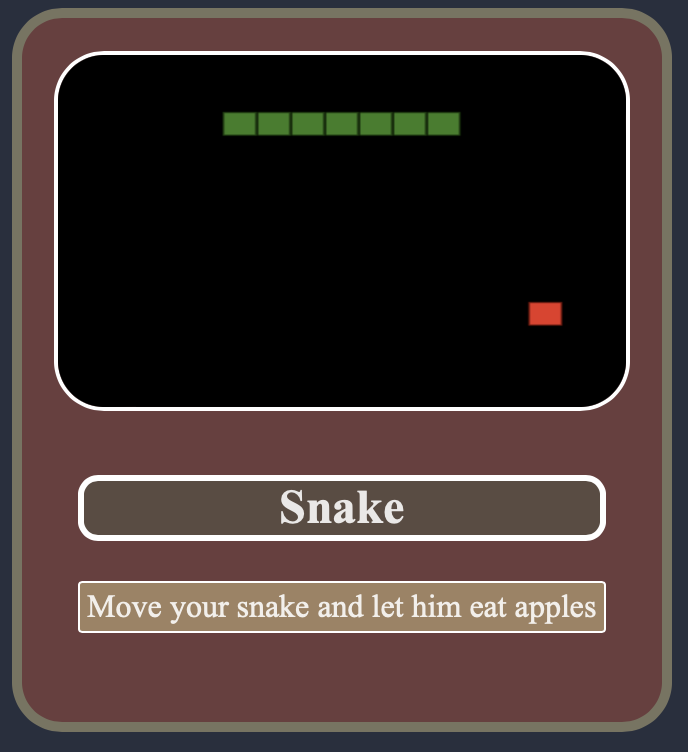
\includegraphics[width=0.9\textwidth]{images/Card.png}
\end{figure}
Questa componente è una semplice scheda utilizzata per indicare i giochi presenti nel sito, è composta da un semplice flexbox
contenente degli elementi paragrafo per il nome e una semplice descrizione e un'immagine.
successivamente questa componenente verrà racchiusa in un componenente link di React-Router-dom che sul click dell'utente 
reindirizza alla pagina del gioco rappresentato. Card è presente solo nella pagina principale del sito.

\subsubsection{Login}
\begin{figure}[H]
    \centering
    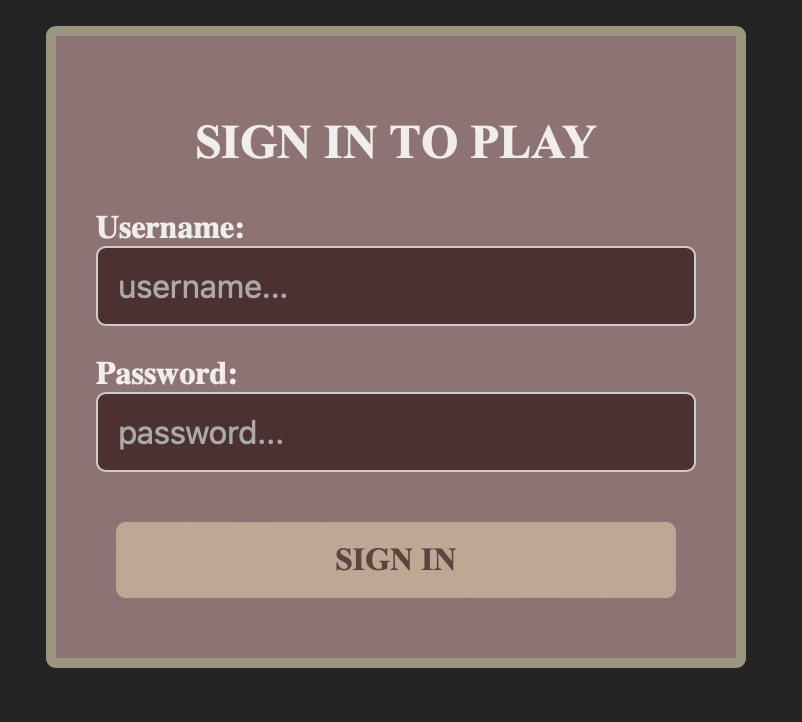
\includegraphics[width=0.9\textwidth]{images/sign_in.png}
\end{figure}
Questa componente è la stessa sia per Login che per Sign in, è molto simile a Card in come si presenta,
tuttavia ha una differenza sostanziale in termini di javascript. il bottone del componente è associato a una funzione chiamata 'handleLogin'

\begin{figure}[H]
    \centering
    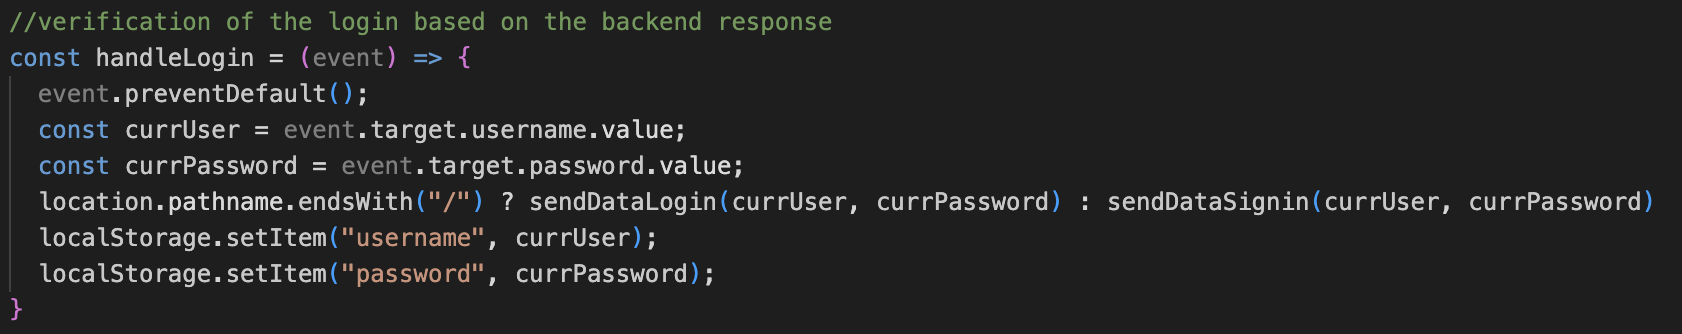
\includegraphics[width=0.9\textwidth]{images/handleLogin.png}
\end{figure}
questa funzione raccoglie i dati inseriti dall'utente nel form e in base alla route, con cui si decide quale delle due versioni del componente utilizzare,
li invia al backend per verificare le credenziali o per creare un nuovo account tramite le due funzioni 'sendDataSignIn' e 'sendDataLogIn' .
come ultima cosa salva i valori inseriti dall'utente nella memoria locale del browser così che siano reperibili in qualunque momento, questi valori sono poi eliminati
dalla funzione di logout in una componente successiva.

Questa componente è montata solo nella pagina iniziale del sito


\subsubsection{Navbar}
\begin{figure}[H]
    \centering
    
\includegraphics[width=0.9\textwidth]{images/Navbar.png}
\end{figure}
Navbar è una componente molto semplice, è composta solo da dei bottoni associati a dei link e uno associato alla funzione di logout prima citata.
Presenta due stati possibili, quando la componente è montata nella pagina principale del sito ha solo due bottoni che collegano le pagine di classifica,
mentre quando è montata in una pagina di classifica, si rende accessibile anche un bottone per ritornare alla pagina principale.
Anche la funzione di logout è molto semplice in quanto elimina solamente i dati dell'utente dalla memoria locale.
Navbar è presente nella pagina principale e nelle pagine di classifica.

\subsubsection{Scoreboard}
\begin{figure}[H]
    \centering
    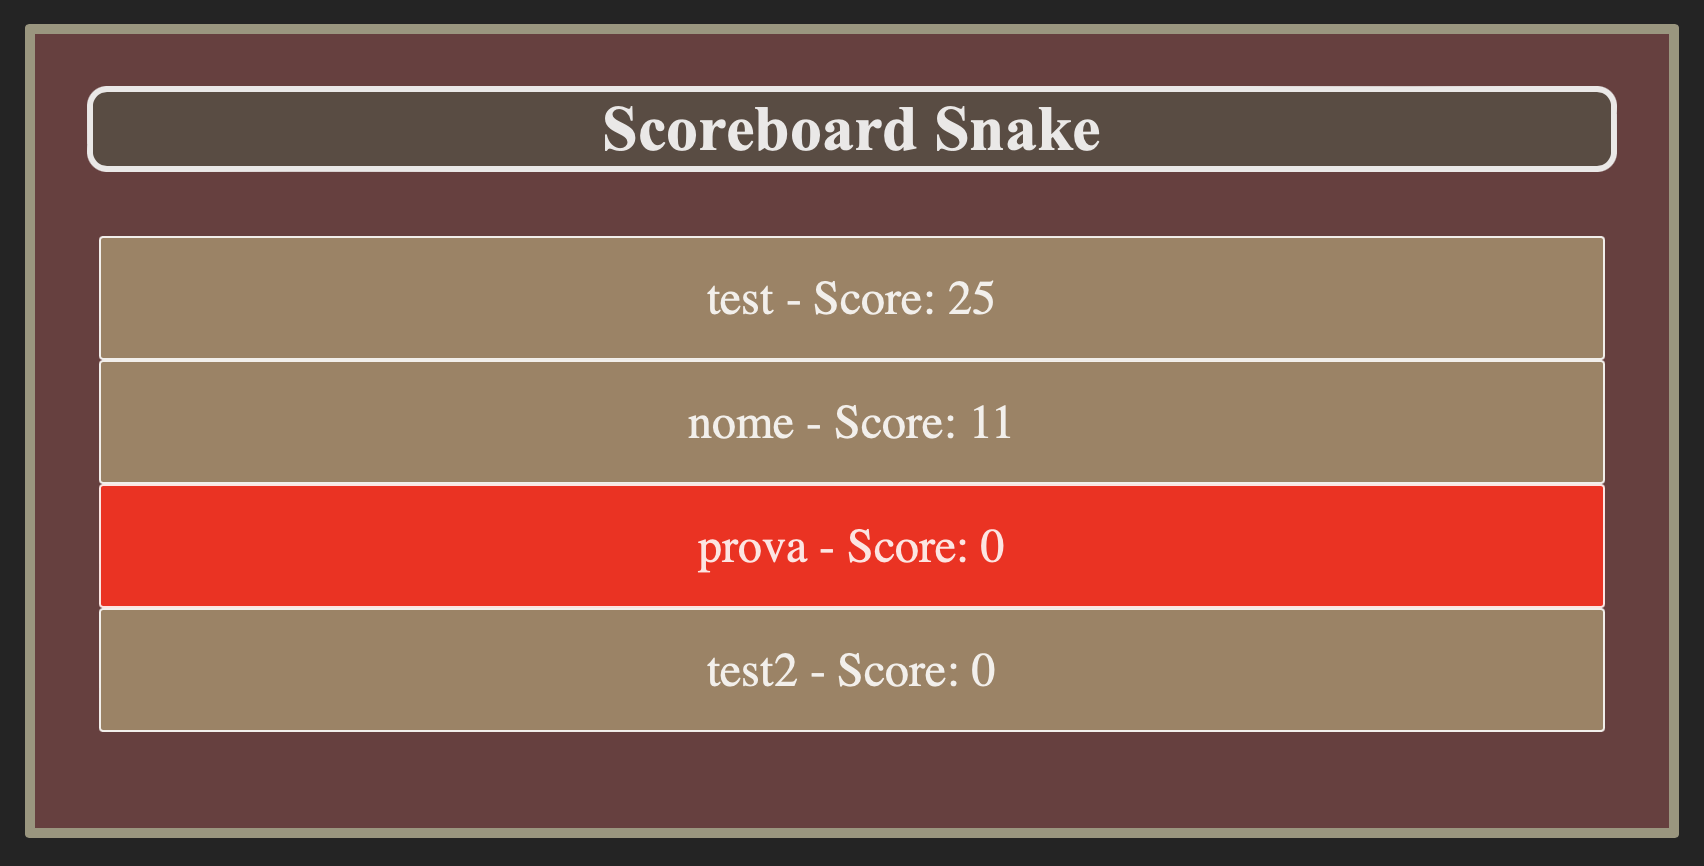
\includegraphics[width=0.9\textwidth]{images/Scoreboard.png}
\end{figure}
Scoreboard è una componente che raccoglie i dati riguardanti un gioco specifico dal backend e li riordina in una lista da presentare all'utente 
illuminando i risultati che lo interessano. L'unico aspetto interessante della componente è come ricava i dati da presentare.
Questo viene fatto tramite Axios, un Client HTTP per node.js, che permette di inoltrare richieste HTTP e ricevere i dati in formato JSON.
Scoreboard è presente solo nelle pagina di classifica.

\subsection{Giochi}
La sezione è dedicata a una analisi più approfondita del funzionamento del codice dei giochi.
Non sono il focus del progetto, in quanto non utilizzano tecnologie particolari se non React.js. La sezione è mirata a facilitare la lettura del codice, se necessario.


\subsubsection{Snake}

\subsubsection{FlappyBird}
Il gioco si basa essenzialmente sul generare degli ostacoli che devono essere evitati dal giocatore. 
Gli ostacoli sono inseriti in una variabile di stato di React e sono renderizzati offscreen ogni 2 secondi.

Innanzitutto si definiscono delle variabili di stato necessarie per il controllo del gioco.
\begin{figure}[H]
    \centering
    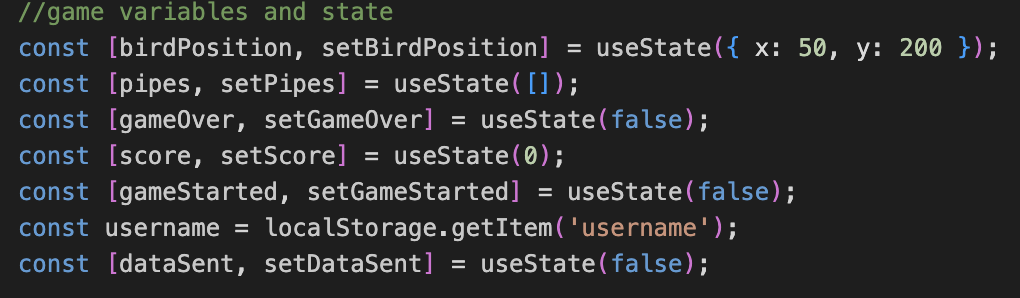
\includegraphics[width=0.9\textwidth]{images/Flappy_variables.png}
\end{figure}


\section{Backend}

\subsection{Import e setup}

\begin{figure}[H]
    \centering
    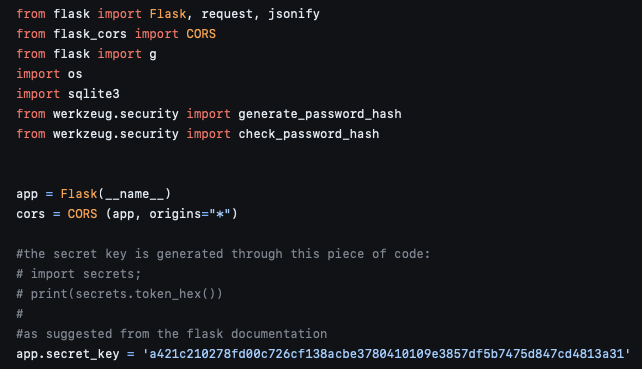
\includegraphics[width=0.9\textwidth]{images/import.png}
\end{figure}

\subsubsection{Import}
Il file inizia con l’import di tutte le librerie verranno utilizzate in seguito: lato server, per la crittografia e per il database.

In particolare viene importato il framework Flask, scelto per la sua semplicità e minimalismo, inoltre si importano tutte le librerie che servono per interagire con il client ricevendo ed inviando rispettivamente con “request" e "jsonify".

La seconda sezione di import riguarda tutto il necessario per il database: g è un oggetto utilizzato per salvare, temporaneamente, e condividere i dati in parti differenti dell' applicazione.

L’import del modulo os serve per gestire la posizione dei file, in particolare del database in questo caso.

Come ultimo import in questa sezione si ha il modulo sqlite3, che consente di creare, inizializzare e utilizzare il database.


Le ultime due righe nella sezione di import servono per i moduli necessari rispettivamente alla creazione e al controllo dell’hash associati alla crittografia della password. 

\subsubsection{Setup di base}
Le prime due righe di codice servono ad inizializzare l' applicazione in flask e a configurare CORS (Cross-Origin Resource Sharing), quest'ultimo serve per consentire richieste da fonti esterne. 
L’asterisco associato al parametro origins specifica che le richieste possano avvenire da qualunque origine (dominio o indirizzo IP).

L’ultima riga di questa sezione è quella che riguarda l’inizializzazione della chiave segreta per la crittografia della password.

\subsection{Setup Database}
Questa sezione di codice, invece, è dedicata alla creazione, inizializzazione e chiusura del database sqlite3, già presente in Flask e ottimo per gestire carichi di lavoro moderati come in questo caso:
\begin{figure}[H]
    \centering
    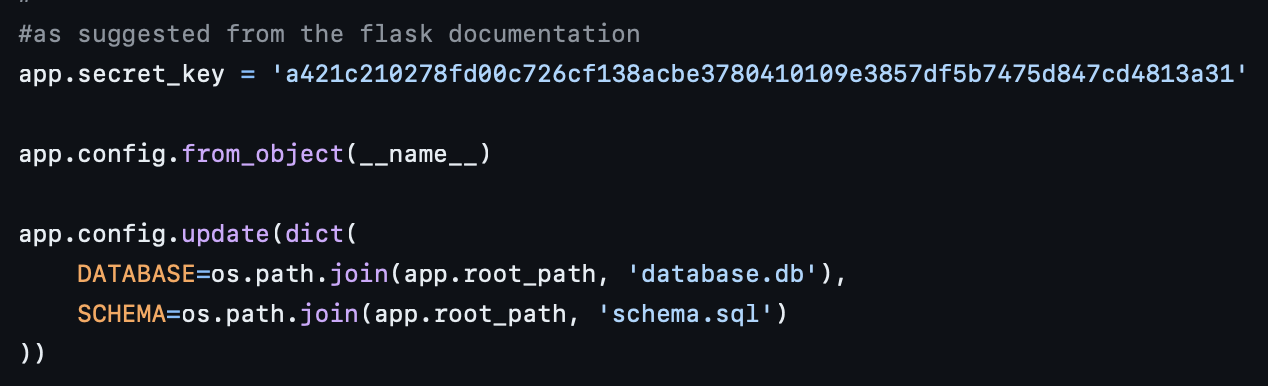
\includegraphics[width=0.9\textwidth]{images/setup_database1.png}
\end{figure}

Questa porzione di codice serve ad impostare quelle che sono le variabili di configurazione per l’inizializzazione e utilizzo del database.

\subsubsection{Connessione con il database}
\begin{figure}[H]
    \centering
    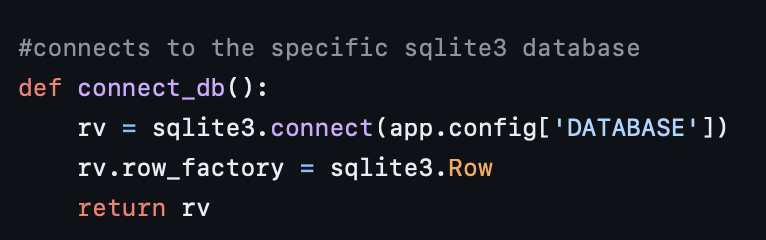
\includegraphics[width=0.9\textwidth]{images/connessione_db.png}
\end{figure}

Questa funzione serve per stabilire una connessione con uno specifico database sqlite3, rv è l’oggetto di connessione al database, che potrà poi essere usato per interagire con lo stesso.

\subsubsection{Aprire una nuova connessione con il database}
\begin{figure}[H]
    \centering
    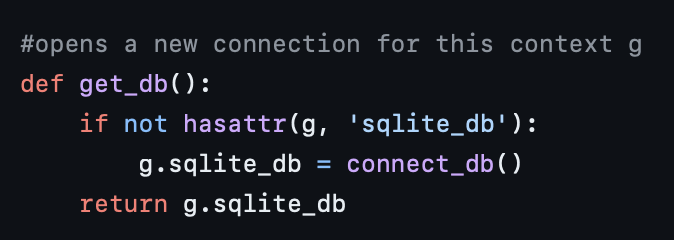
\includegraphics[width=0.9\textwidth]{images/apertura_connessione_db.png}
\end{figure}

Funzione che permette, nel caso non fosse già presente, di instaurare una nuova connessione e memorizzarne il contenuto nell’oggetto g, permettendo così di utilizzarla in diverse parti dell’applicazione.

\subsubsection{Chiusura della connessione}
\begin{figure}[H]
    \centering
    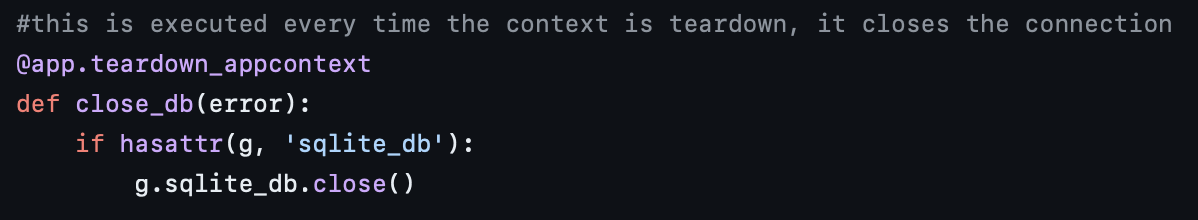
\includegraphics[width=0.9\textwidth]{images/chiusura_connessione_db.png}
\end{figure}

Questa funzione invece serve per concludere la connessione con il database allorché l’applicazione Flask termini di utilizzarlo, in modo da evitare problemi di risorse non rilasciate.

\subsubsection{Inizializzazione del database}
\begin{figure}[H]
    \centering
    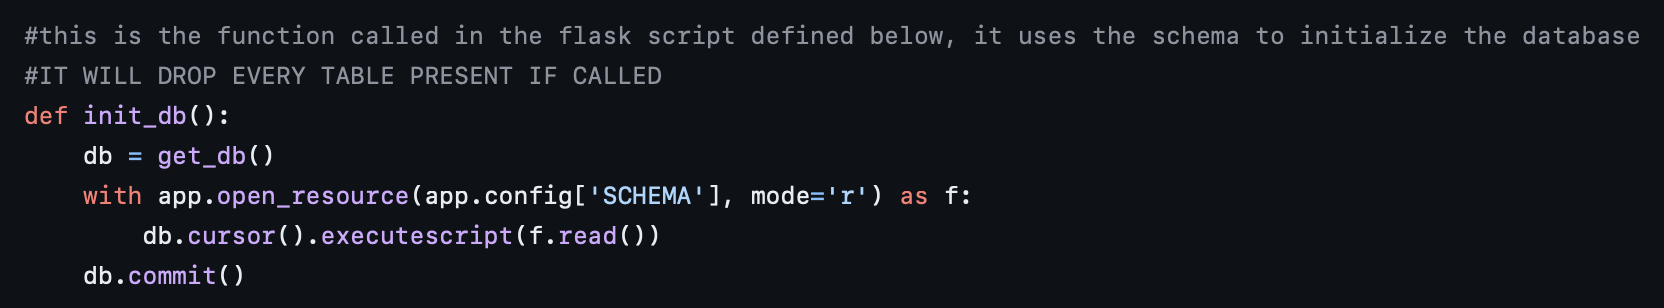
\includegraphics[width=0.9\textwidth]{images/inzializzazione_db.png}
\end{figure}

Questa funzione serve per inizializzare il database all’interno dell’applicazione Flask: prima si invoca la funzione get\textunderscore db in modo da ottenere la connessione con il database, poi si apre il file dello schema, in modalità lettura.
Dopo aver ottenuto un oggetto cursos, questo si utilizza per eseguire lo script letto nel file schema.sql; db.commit confermare le modifiche appena fatte.



\subsubsection{Inizializzazione da linea di comando}
\begin{figure}[H]
    \centering
    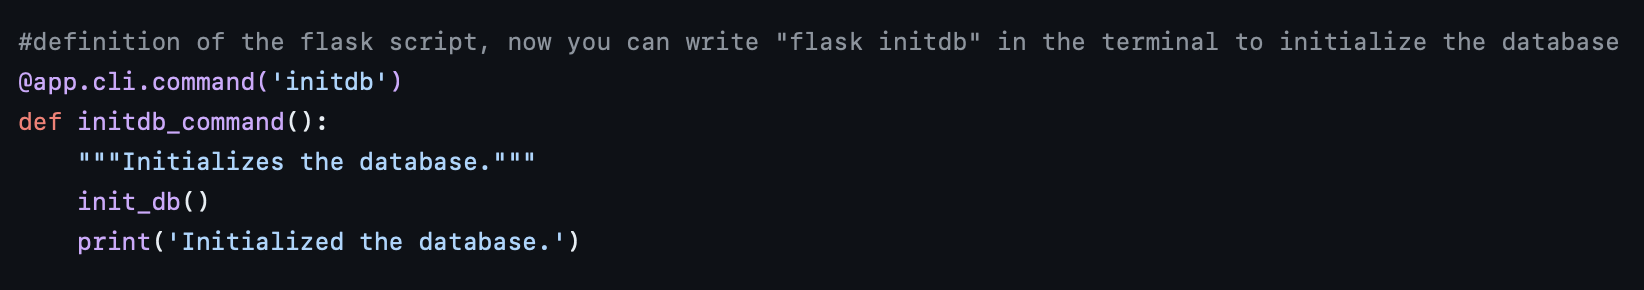
\includegraphics[width=0.9\textwidth]{images/inizializzazione_linea_comando.png}
\end{figure}

Quest’ultima porzione di codice, per quanto riguarda la sezione dedicata al database, permette di inizializzare il database tramite linea di comando “flask initdb”. 
Una volta dato questo comando il database sarà inizializzato e pronto per essere utilizzato.

Da tenere in considerazione che tutte le volte che questo comando viene lanciato il database sarà azzerato, perdendo tutti i dati al proprio interno.


\subsection{API}
Questa sezione è dedicata alle API, funzioni che permettono di comunicare con il client e nelle quali si utilizza effettivamente il database creato nella porzione precedente di codice.

\subsubsection{Invio della classifica}
\begin{figure}[H]
    \centering
    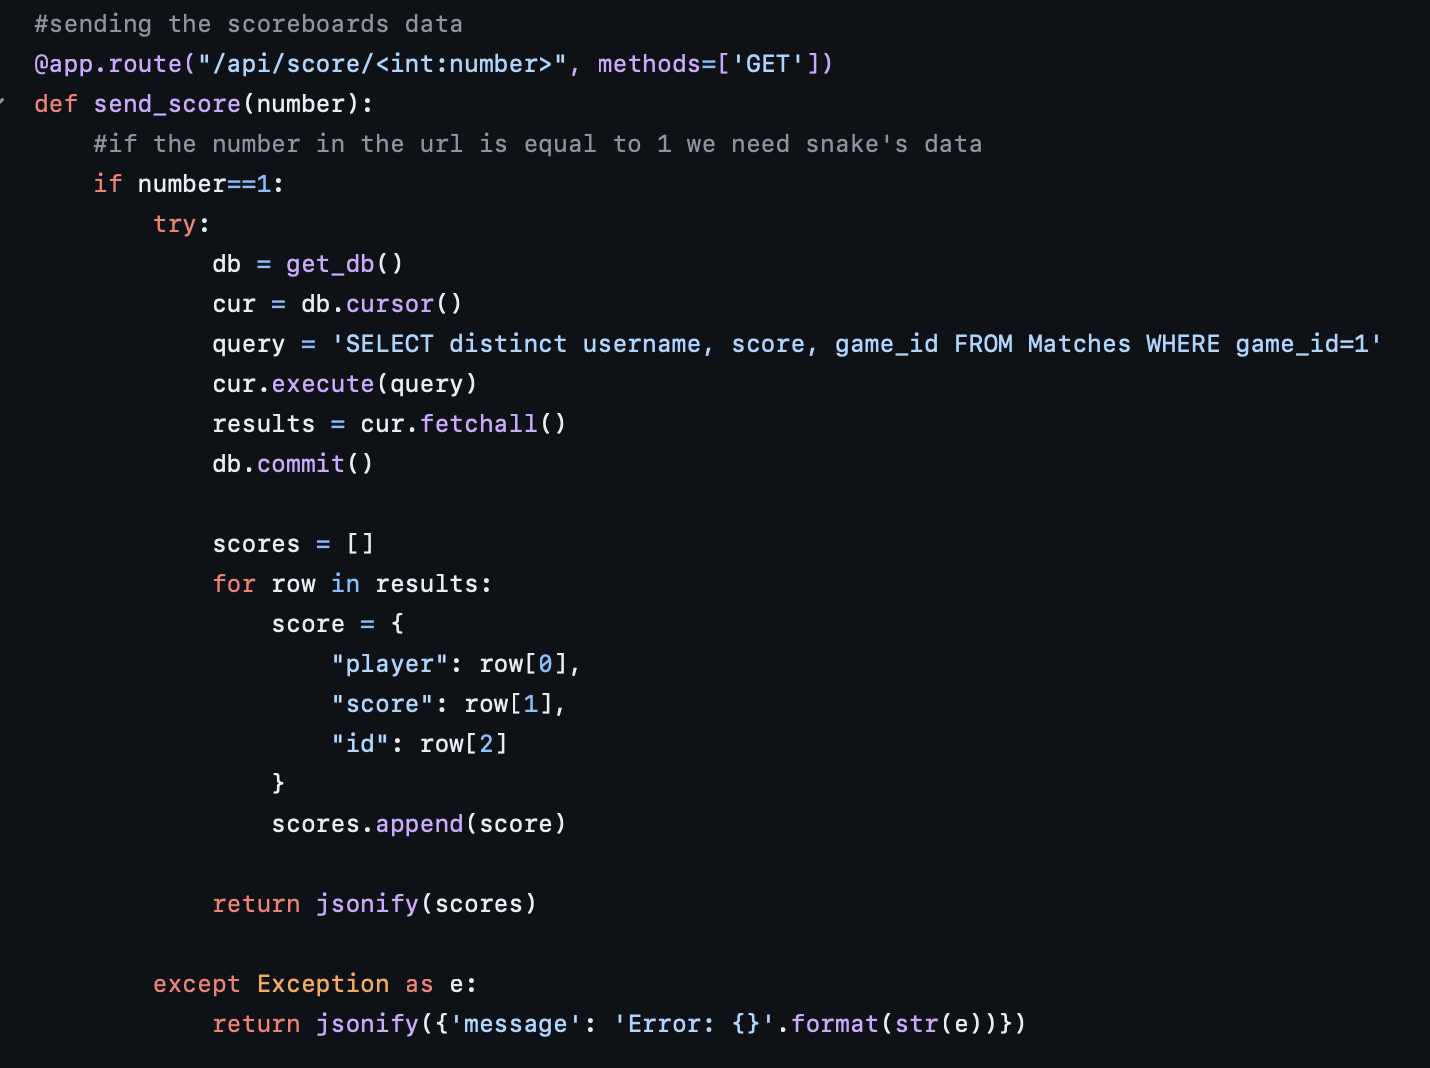
\includegraphics[width=0.9\textwidth]{images/invio_classifica1.png}
\end{figure}

\begin{figure}[H]
    \centering
    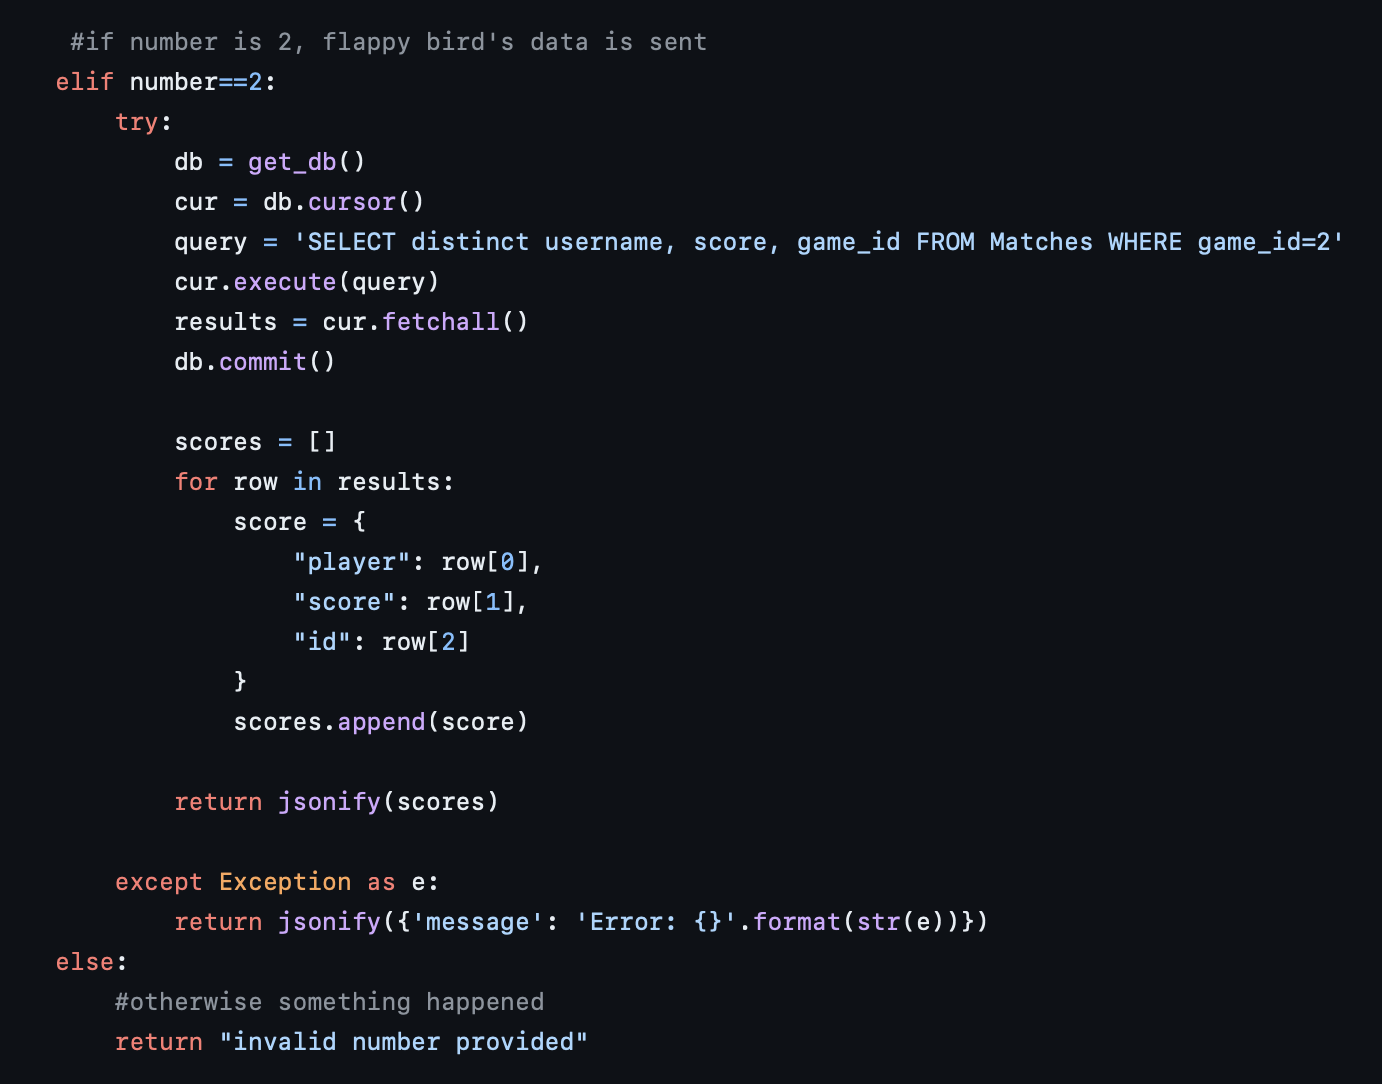
\includegraphics[width=0.9\textwidth]{images/invio_classifica2.png}
\end{figure}
Questa funzione di tipo GET, che quindi invia dati dal server al client, serve per inviare i punteggio, id del gioco, e nome utente, legati tra loro, tenuti nel database, al client in modo da poter mostrare le classifiche divise per gioco.

La richiesta del client avviene ad un url specifico che termina con un valore numero intero, tale valore numerico assume un valore differente per specificare di quale gioco si vuole ricevere i punteggi.

Una volta identificato il gioco, tramite un semplice if statement, si utilizzano le funzioni per instaurare la connessione con il database per poter effettuare la query ed estrarre le informazioni necessarie dal database.

Tutte le tuple ottenute sono salvate in una variavbile, tramite il metodo fetchll, che che consente di tenere tutti i risultati e non solo uno, poi una lista di json viene creata con i risultati ottenuti; lista che poi sarà al client tramite apposito metodo.

Il tutto viene fatto in regime di try catch per intercettare un qualunque errore che potrebbe avvenire e notificare di conseguenza il client.

\subsubsection{Salvare il punteggio delle partite}

\begin{figure}[H]
    \centering
    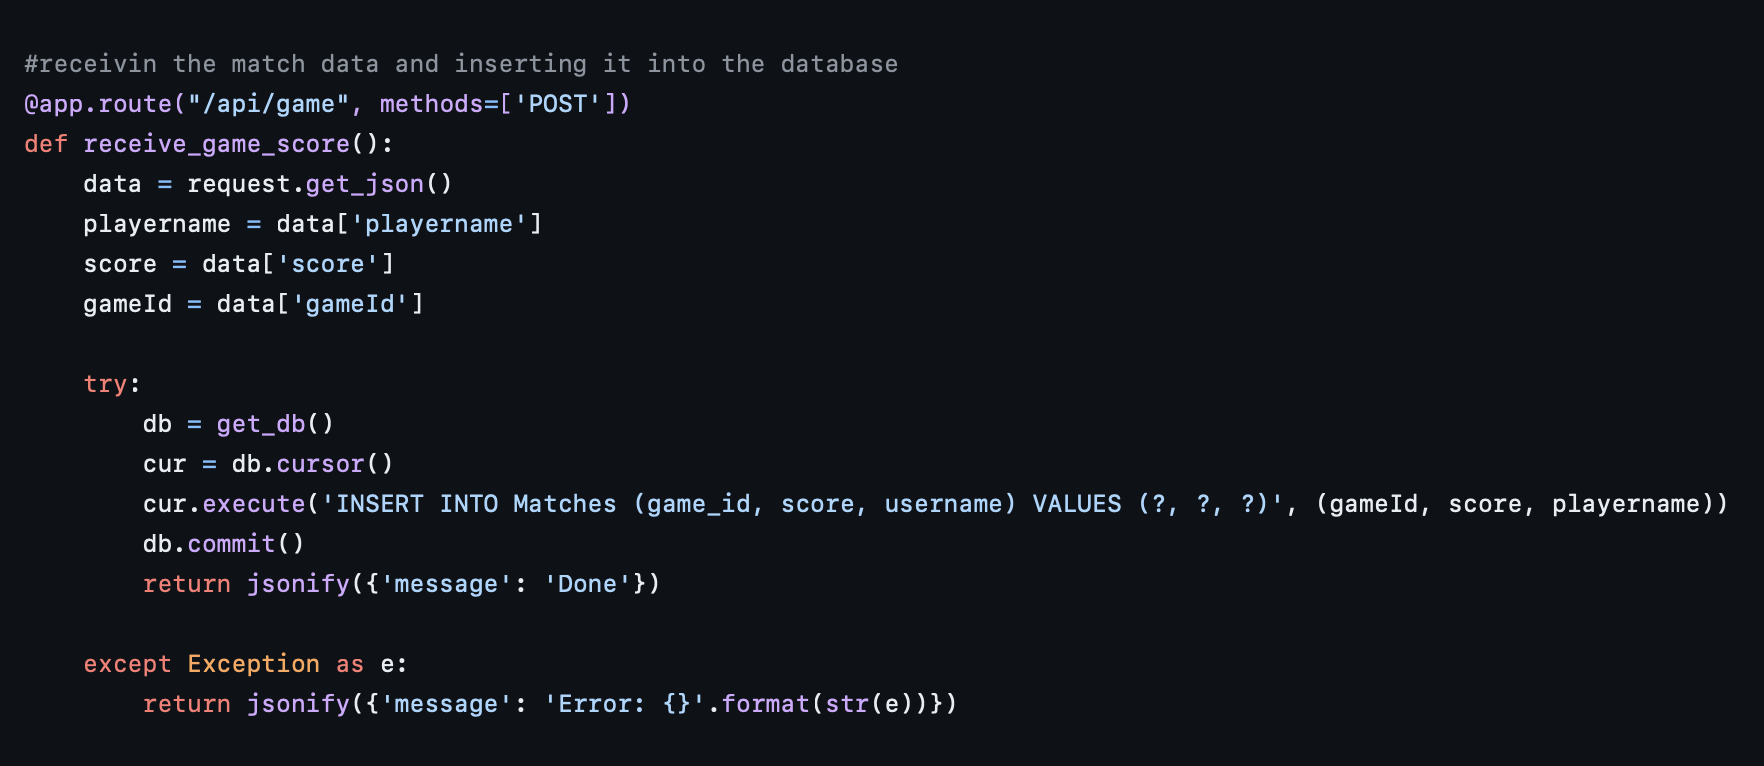
\includegraphics[width=0.9\textwidth]{images/salvare_punteggio_partite.png}
\end{figure}
Questa funzione di tipo POST, che quindi invia dati dal client al server, serve per ricevere e i dati ottenuti da una partita giocata; i dati passati dal client in formato json vengono poi messi nel database tramite la funzione INSERT. 

Queste operazioni vengono tutte eseguite in regime di try catch in modo da intercettare un qualunque errore e notificare il client sia in caso di operazione performata con successo, sia in caso in cui sia avvenuto un errore.

\subsubsection{Controllo accesso di un utente}
\begin{figure}[H]
    \centering
    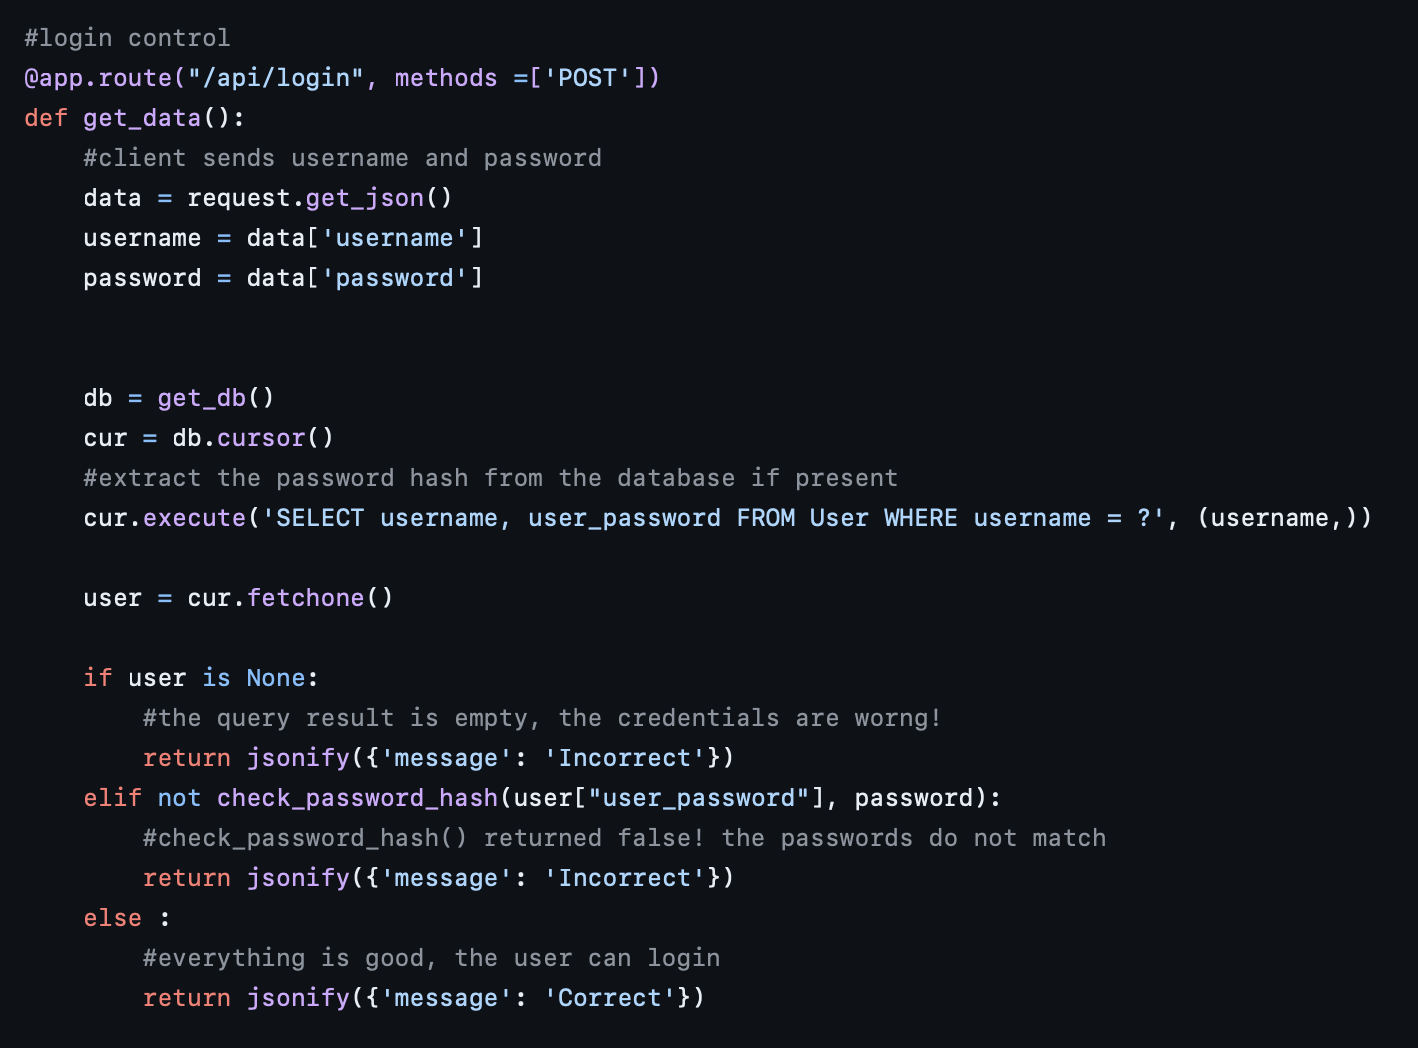
\includegraphics[width=0.9\textwidth]{images/controllo_login.png}
\end{figure}

Questa funzione serve per permettere l’accesso ad utente già registrato.
La funzione riceve dal client il nome utente e la password inseriti: per prima cosa controlla che lo username esista, se esiste allora controlla che anche la password, dopo aver usato l’apposita funzione per decriptarla, corrisponda.
Il nome utente è univoco essendo chiave primaria nello schema sql, motivo per cui si usa la fatchone e non la fatchall.

Al termine il client é notificato con il risultato ottenuto dalla verifica.

\subsubsection{Iscrizione nuovo utente}
\begin{figure}[H]
    \centering
    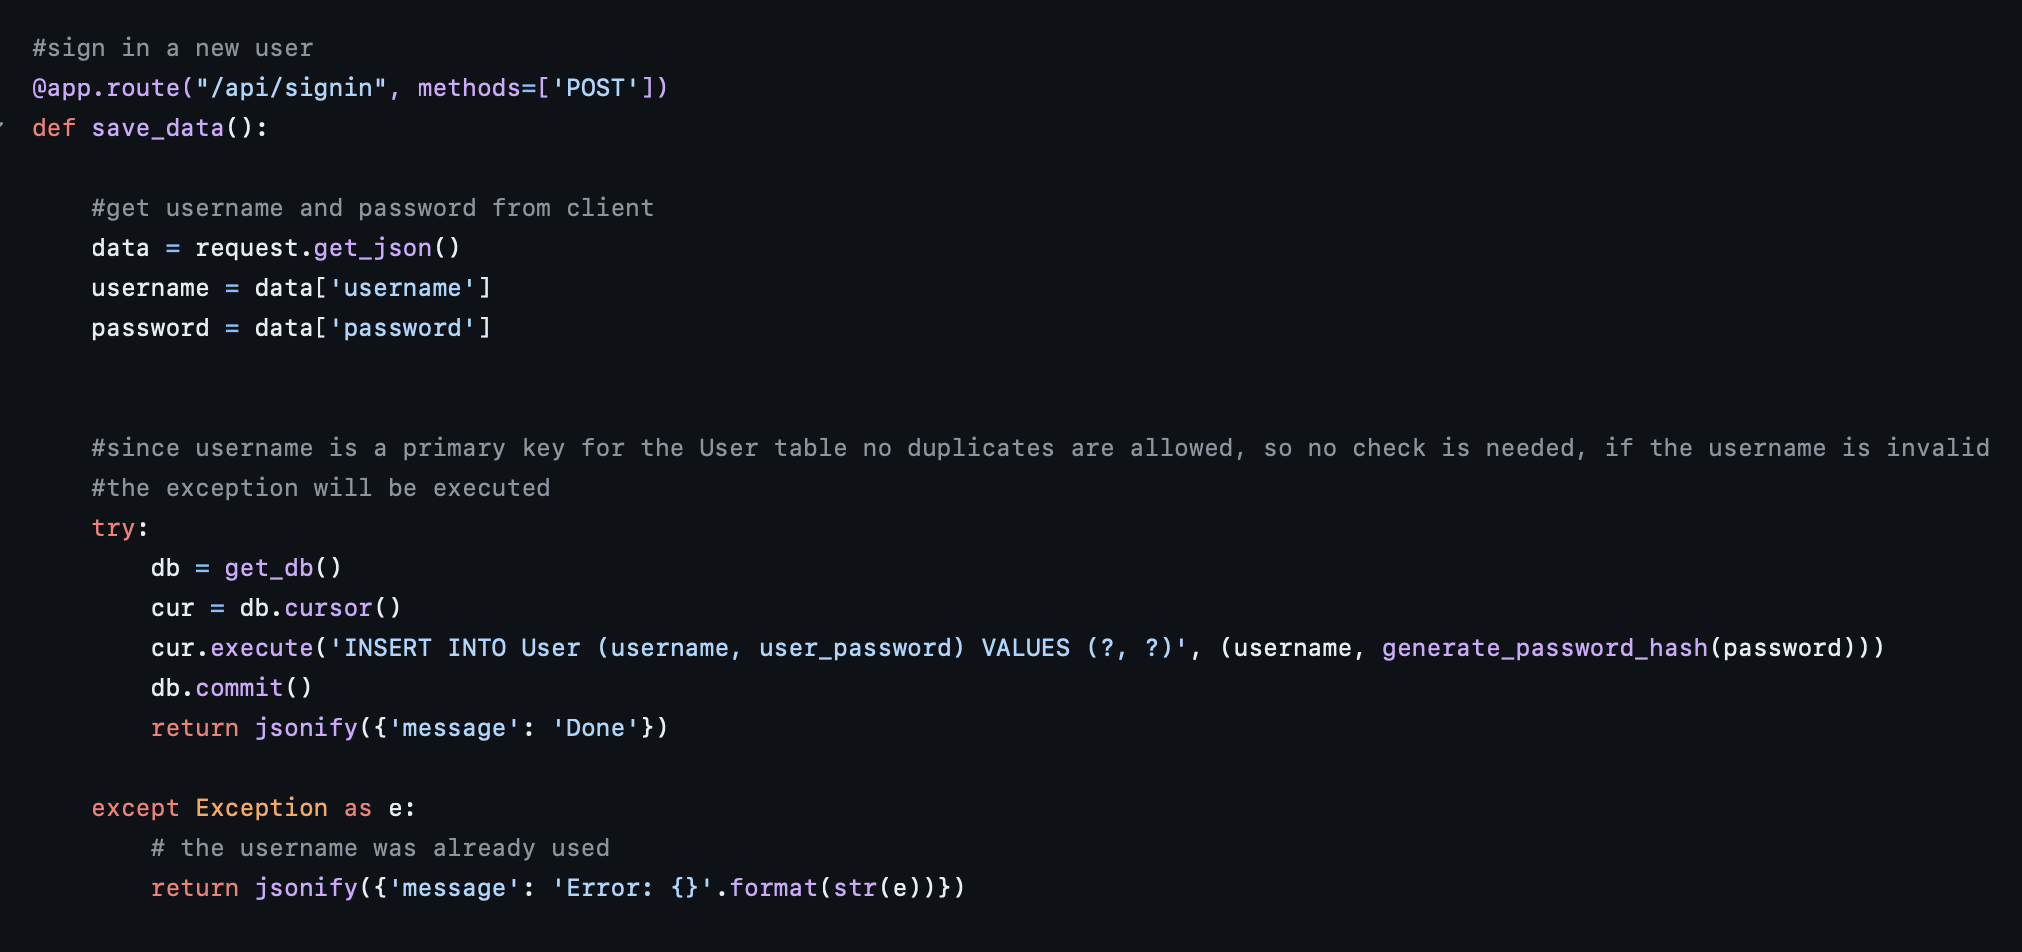
\includegraphics[width=0.9\textwidth]{images/iscrizione_nuovo_utente.png}
\end{figure}

Questa funzione è quella per permette ad un nuovo utente di iscriversi: riceve ancora una volta il nome utente e la password dal client in formato json, dopo di che aggiunge questi valori al database.
L’unico errore che può verificarsi è che il nome utente sia già presente nel database, essendo chiave primaria non possono essere presenti due nomi utenti uguali, in tal caso il client è notificato che l’operazione richiesta non è andata a buon fine.

\subsubsection{Invio informazioni giochi}
\begin{figure}[H]
    \centering
    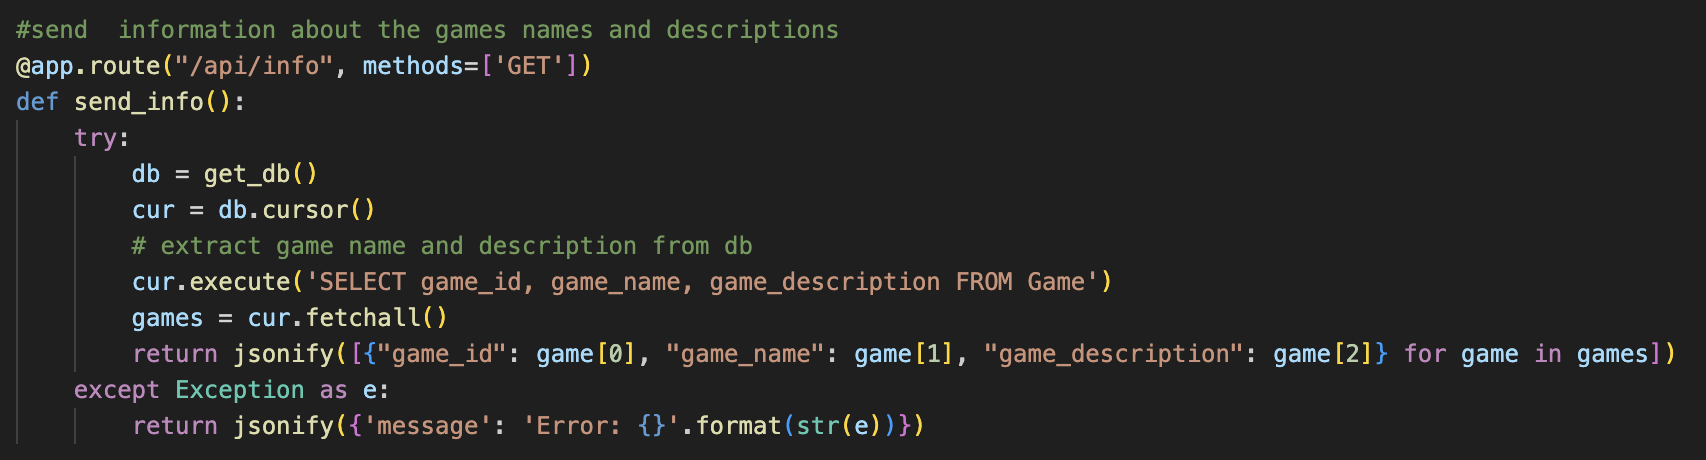
\includegraphics[width=0.9\textwidth]{images/game_info.png}
\end{figure}
Quest'ultima funzione serve per inviare le informazioni relative ai giochi.
Esegue una query per estrarre tutte le informazioni a disposizione nel datbase e poi le invia al client in formato JSON. 

\subsubsection{Sezione dedicare all'esecuzione dell'app (facoltativa)}
\begin{figure}[H]
    \centering
    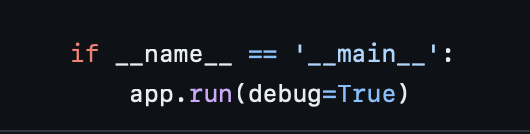
\includegraphics[width=0.9\textwidth]{images/esecuzione_app.png}
\end{figure}

Queste sono le due ultime righe del backend e sono facoltative: ci servono solo per avviare la nostra applicazione e farlo con la modalità debug attiva.



\subsection{Database}
Il database in sqlite3 ha una struttura relazionale e si basa su tre tabelle sql.
\begin{figure}[H]
    \centering
    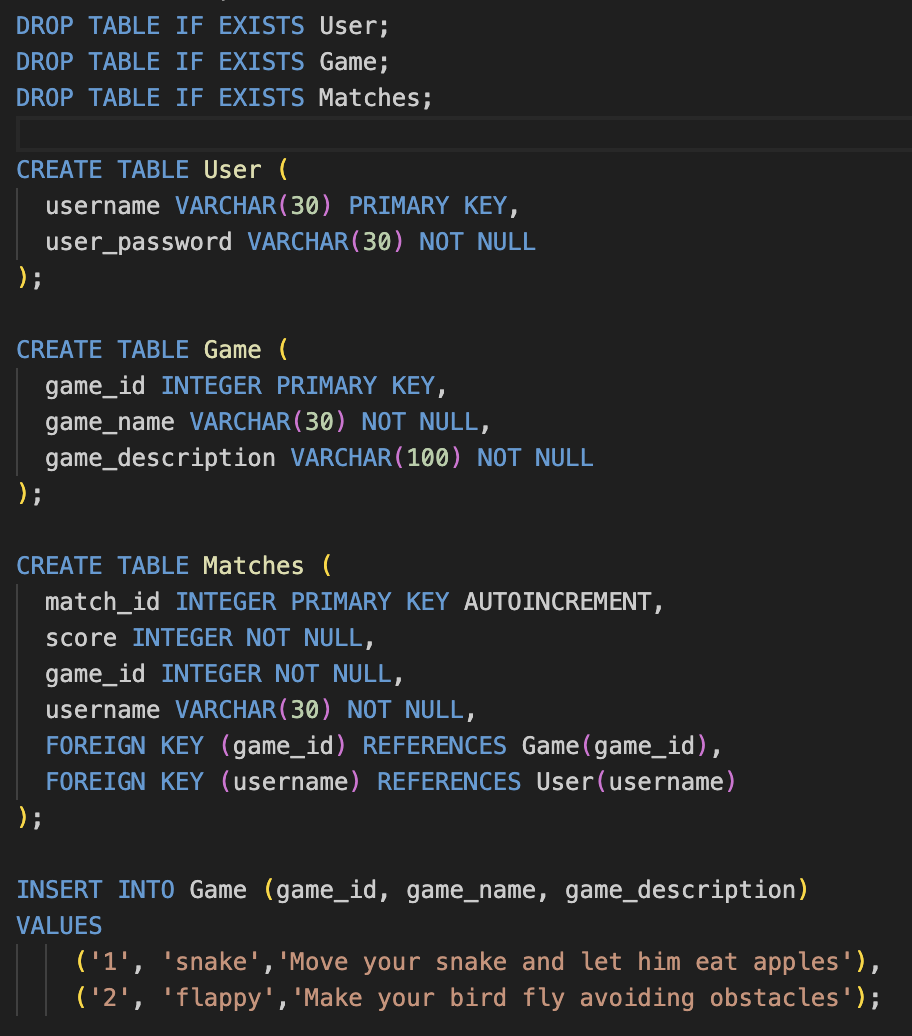
\includegraphics[width=0.9\textwidth]{images/schema_db.png}
\end{figure}

sono create 3 tabelle: User, Game e Matches.

La tabella User è quella che contiene il nome utente e la password di ogni utente; essendo username chiave primaria questo evita che ci possano essere due utenti con lo stesso nome.

Game invece contiene l’id identificativo associato a ciascun gioco (1 per snake e 2 per flappy), il nome del gioco e la sua descrizione. 
Viene inizializzato direttamente con questi valori al suo interno quando viene creato il database.

Matches è invece la tabella che si occupa di mettere in relazione le altre due: infatti contiene sia lo username che il game\textunderscore id e in aggiunta il match\textunderscore id, valore che identifica in modo univoco ogni partita giocata, e il punteggio ottenuto in tale partita. 
Infine sono esplicitati i vincoli di integrità referenziale.





\end{document}